\documentclass{beamer}

\usepackage{beamerthemesplit} %Activate for custom appearance
\usepackage{wrapfig}
\usepackage{amsmath}
\usepackage{amsfonts}
\usepackage{amssymb}
\usepackage{amsthm}
%\usepackage[outdir=./]{epstopdf}
\usepackage{mathbbol}
%\usepackage{tikz}
\usepackage{color}
\usepackage[ruled]{algorithm}
\usepackage{algorithmic}
\usepackage{multirow}
\usepackage{graphicx}
\usepackage{xkeyval}
\usepackage{todonotes}
\presetkeys{todonotes}{inline}{}
\usepackage{arydshln}
\usepackage{caption} 
\usepackage{subcaption}
\usepackage{verbatim}
\definecolor{DeepSkyBlue}{rgb}{0.6,0.6,1}
\setbeamercolor{eecks} {bg=DeepSkyBlue, fg=black!10}
\setbeamercolor{eeks2}{bg=black!8, fg=black}

\mode<presentation>{%
  \usetheme{Boadilla}
}

\usefonttheme[onlymath]{serif}
\newenvironment{ovalboxpage}[1]{\begin{center}\begin{minipage}{#1}\begin{block}{}}{\end{block}\end{minipage}\end{center}}
\newenvironment{ovalboxpagetitle}[2]{\begin{center}\begin{minipage}{#1}\begin{block}{#2}}{\end{block}\end{minipage}\end{center}}
\newenvironment{obpt}[1]{\begin{center}\begin{minipage}{0.95\textwidth}\begin{block}{#1}}{\end{block}\end{minipage}\end{center}}
\newenvironment{obptsmall}[1]{\begin{center}\begin{minipage}{0.6\textwidth}\begin{block}{#1}}{\end{block}\end{minipage}\end{center}}

\newcommand{\R}{\mathbb{R}}

\title[Fast Somewhat Accurate Algorithms]{Fast and Somewhat Accurate Algorithms (Team 4)}
\author[Team 4]{Mario Barela, Su Chen,
Emily Gunawan,
Morgan Schreffler, Minho Song,
Doyeob Yeo, with mentor:
Chai Wah Wu (IBM)}
\date[Final Presentation]{Friday, August 14, 2015}
\institute[IMA]{IMA: Modeling in Industry Final Presentation}

\begin{document}
\begin{frame}
\titlepage % Print the title page as the first slide
\end{frame}


\begin{frame}
\frametitle{Outline}
  \begin{figure}[htb]
  \begin{center}
  \mbox{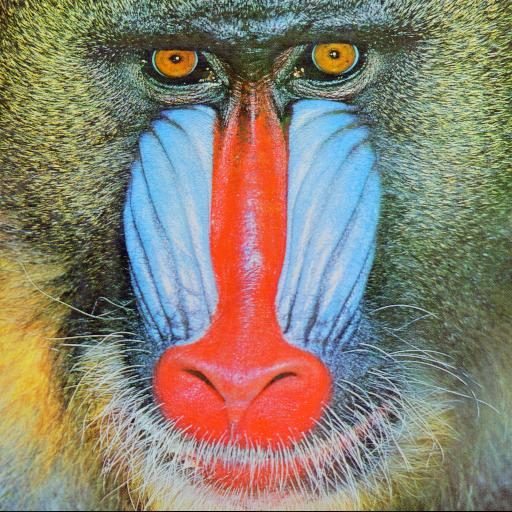
\includegraphics[height=1in]{BaboonRGB.jpg}}
\mbox{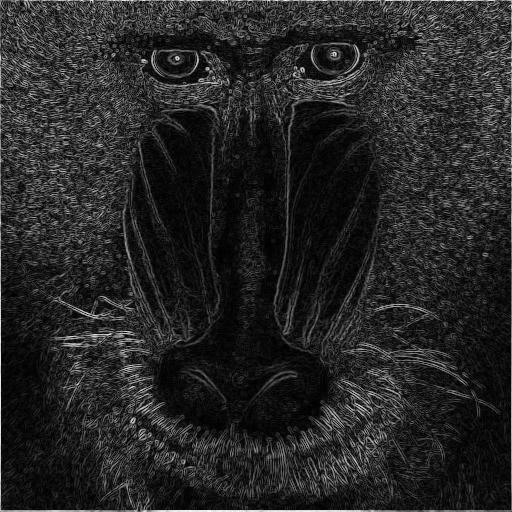
\includegraphics[height=1in]{Baboon_after_sobel_magnitude.jpg}}
\mbox{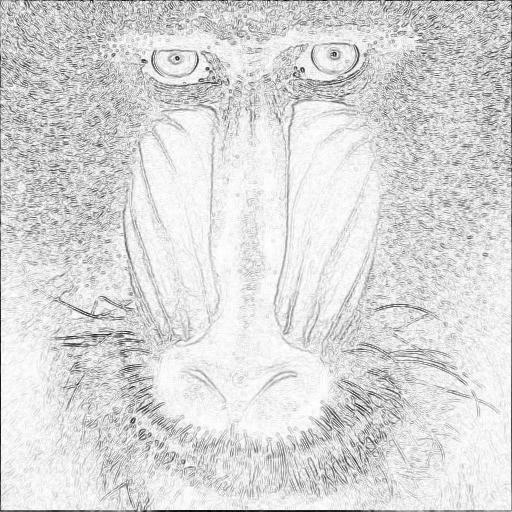
\includegraphics[height=1in]{Baboon_after_sobel_magnitude_inverse.jpg}}
  % Mandrill 
 
  \end{center}
  \end{figure}
% Table of contents slide, comment this block out to remove it

\tableofcontents % Throughout your presentation, if you choose to use \section{} and \subsection{} commands, these will automatically be printed on this slide as an overview of your presentation
\end{frame}

\section{Motivation/Problem}

\begin{frame}
\frametitle{Problem}
We study the tradeoff between accuracy and system complexity as measured by processing speed and hardware complexity.

\end{frame}

\begin{comment}
\begin{frame}
\frametitle{Where is image processing used?}
\begin{figure}[htb]
  \begin{center}  \mbox{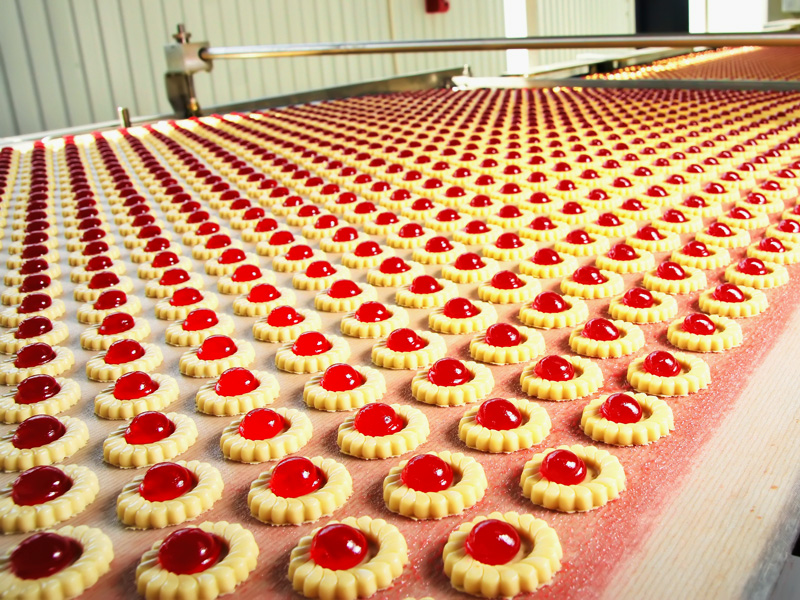
\includegraphics[height=1in]{Quality_Control.jpg}}
   \mbox{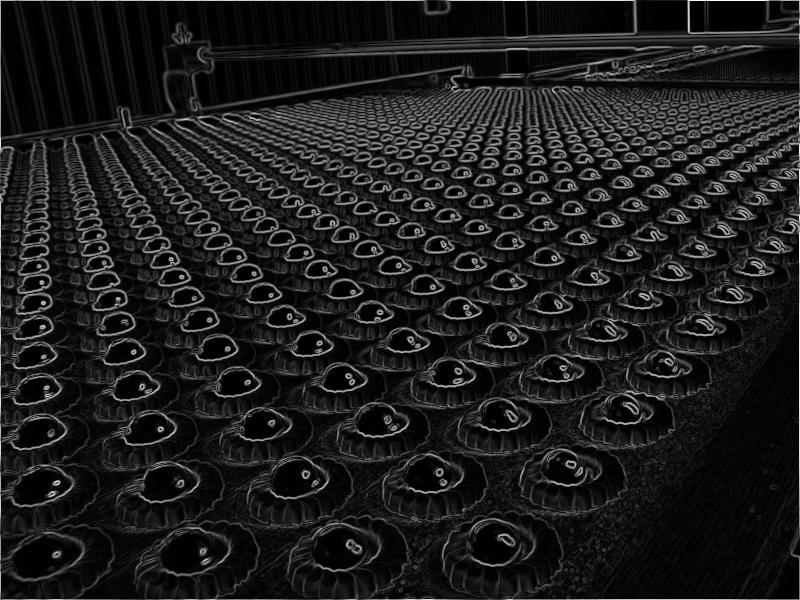
\includegraphics[height=1in]{Quality_Control_after_sobel_magnitude.jpg}}
 \mbox{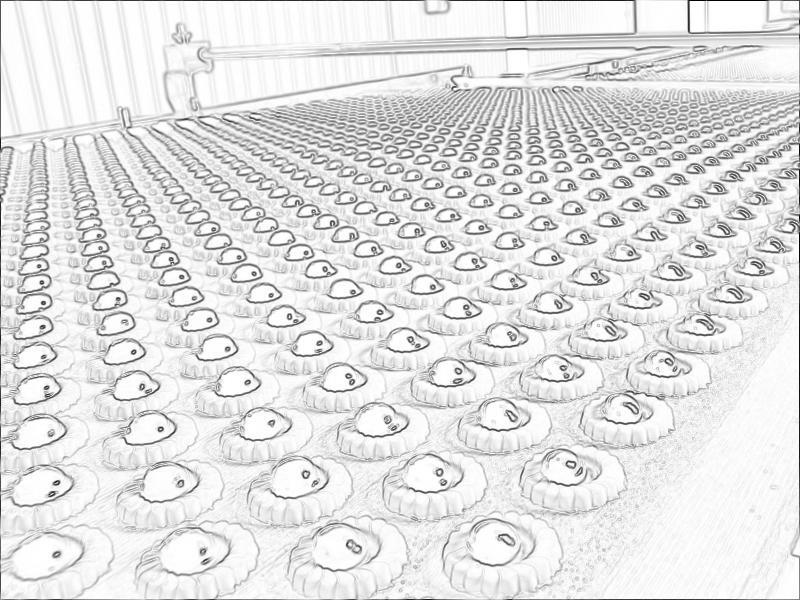
\includegraphics[height=1in]{Quality_Control_after_sobel_magnitude_inverse.jpg}}
  \caption{Pastry industry quality control}
  \end{center}
  \end{figure}
  
\begin{itemize}
%\item Quality Control 
\item
Computer vision (license plate reader, tracking human motion)
\item
Optical imaging (cameras, microscopes)
\item
Medical imaging (MRI, ultrasound) %, %astronomical imaging (telescopes)
\item
Geophysical imaging, printing
\end{itemize}
\end{frame}

\section{Filtering an Image}

\begin{frame}
\frametitle{An edge-detection filter example}

\todo{Emily writes: this slide is not necessary. To save time, this slide can be removed/replaced.}
\begin{figure}[htb]
  \begin{center}
  \mbox{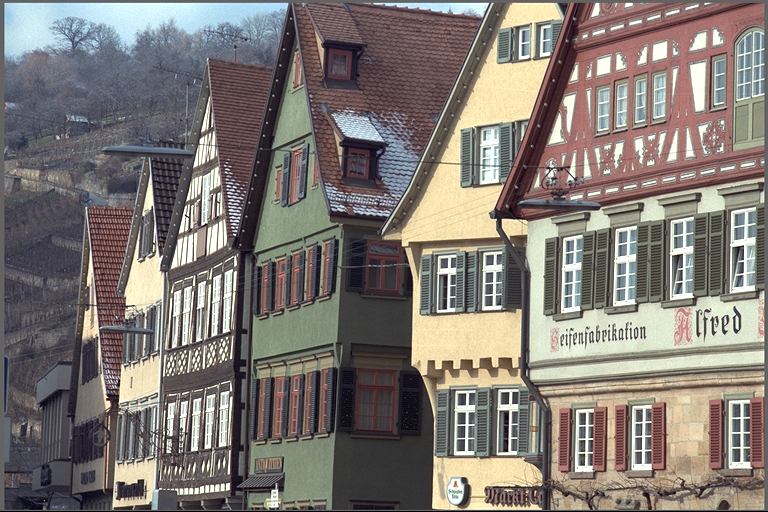
\includegraphics[height=1in]{german.png}}
   \mbox{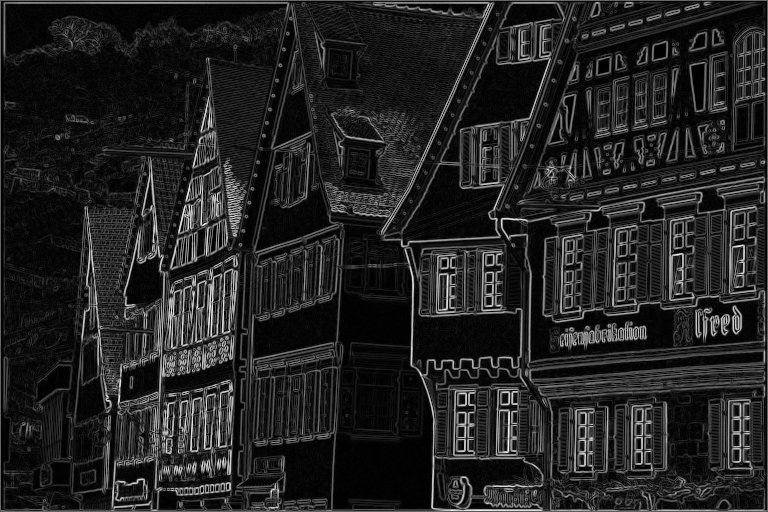
\includegraphics[height=1in]{german_after_sobel_magnitude.png}}
   
 \mbox{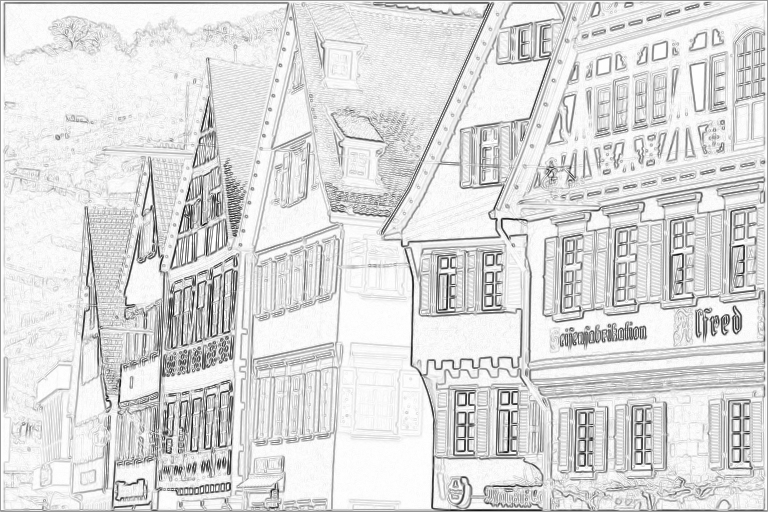
\includegraphics[height=1in]{german_after_sobel_magnitude_inverse.png}}  
%  \caption{German houses from Kodak}
  \end{center}
\end{figure}

\end{frame}


\begin{frame}
\frametitle{Kernel Convolution $\text{IMAGE}*K$}
\todo{Emily writes: I think this slide (and the next one) is not the best. I don't care if this slide (and the next slide) is removed/replaced.}

\begin{itemize}
\item A \emph{convolution matrix} % or kernel, or mask
is a small matrix used for filtering an image.
\item $\text{IMAGE}=
\begin{bmatrix}
\textcolor{blue}{a} & \textcolor{blue}{b} & \textcolor{blue}{c} & d \\
\textcolor{blue}{e} & \textcolor{red}{g} & \textcolor{blue}{h} & i\\
\textcolor{blue}{j} & \textcolor{blue}{m} & \textcolor{blue}{n} & p
\end{bmatrix}$
and
$
K = \begin{bmatrix}
{0} & {-1} & {0}\\
{-1} & {4} & -1\\
{0} & {-1} & {0}
\end{bmatrix}$

\item %To compute the new pixel value at the location of \textcolor{red}{$g$},
%we put the flipped kernel $F$ on top of
To compute the new value at pixel % at the location of
\textcolor{red}{$g$},
place $K$ on top of 
$\text{IMAGE}$, centered at $\textcolor{red}{g}$.
Perform point-wise multiplications and sum up the results:\\

$\begin{bmatrix}
0(a) & -1(b) & 0(c) \\
-1(e) & 4\textcolor{red}{(g)} & -1(h) \\
0(j) & -1(m) & 0(n) 
\end{bmatrix}$

\bigskip

\item The pixel \textcolor{red}{$g$} is replaced by:
$-b-e+4\textcolor{red}{g}-h-m.$

\end{itemize}
\end{frame}


\begin{frame}
\frametitle{Kernel Convolution $\text{IMAGE}*K$}
%$IMAGE
$
\tiny
\begin{bmatrix}
\textcolor{blue}{a} & \textcolor{blue}{b} & \textcolor{blue}{c} & d \\
\textcolor{blue}{e} & \textcolor{red}{g} & \textcolor{blue}{h} & i\\
\textcolor{blue}{j} & \textcolor{blue}{m} & \textcolor{blue}{n} & p
\end{bmatrix}
*\tiny{\begin{bmatrix}
0 & -1 & 0\\
-1 & 4 & -1\\
0 & -1 & 0
\end{bmatrix}}=$
\tiny
 \[
\arraycolsep=0.6pt\def\arraystretch{2.9}
\left[ 
\begin{array}{c@{}c@{}c@{}c}
\begin{array}{ccccc}
0(0) &+& 0(-1) &+& 0(0)+\\ 
0(-1) &+& a(4) &+& b(-1)+\\
0(0) &+& e(-1) &+& g(0)\\
\end{array}
  & 
\left| \begin{array}{ccccc}
0(0) &+& 0(-1) &+& 0(0)+\\ 
a(-1) &+& b(4) &+& c(-1)+\\
e(0) &+& g(-1) &+& h(0)\\
\end{array}\right| 
  & 
\begin{array}{ccccc}
0(0) &+& 0(-1) &+& 0(0)+\\ 
g(-1) &+& h(4) &+& i(-1)+\\
m(0) &+& n(-1) &+& p(0)\\
\end{array} 
  & 
  \left|
\begin{array}{ccccc}
0(0) &+& 0(-1) &+& 0(0)+\\ 
h(-1) &+& i(4) &+& 0(-1)+\\
n(0) &+& p(-1) &+& 0(0)\\
\end{array} 
\right|
\\ \hdashline % end of first row
\begin{array}{ccccc}
0(0) &+& a(-1) &+& b(0) +\\ 
0(-1) &+& e(4) &+& g(-1) +\\
0(0) &+& j(-1) &+& m(0) \\
\end{array} 
&
\left|  
\textcolor{red}{
\begin{array}{ccccc}
a(0) &+& b(-1) &+& c(0) +\\ 
e(-1) &+& g(4) &+& h(-1) +\\
j(0) &+& m(-1) &+& n(0) \\
\end{array}}\right| 
& 
\textcolor{black}{
\begin{array}{ccccc}
b(0) &+& c(-1) &+& d(0) +\\ 
g(-1) &+& h(4) &+& i(-1) +\\
m(0) &+& n(-1) &+& p(0) \\
\end{array} }
& 
\left|
\begin{array}{ccccc}
c(0) &+& d(-1) &+& 0(0) +\\ 
h(-1) &+& i(4) &+& 0(-1) +\\
n(0) &+& p(-1) &+& 0(0)\\
\end{array} 
\right|
\\ \hdashline % end of second row
\begin{array}{ccccc}
0(0) &+& e(-1) &+& g(0) +\\ 
0(-1) &+& j(4) &+& m(-1) +\\
0(0) &+& 0(-1) &+& 0(0)\\
\end{array} 
& 
\left| \begin{array}{ccccc}
e(0) &+& g(-1) &+& h(0) +\\ 
j(-1) &+& m(4) &+& n(-1) +\\
0(0) &+& 0(-1) &+& 0(0) \\
\end{array} \right| 
&
\begin{array}{ccccc}
g(0) &+& h(-1) &+& i(0) +\\ 
m(-1) &+& n(4) &+& p(-1) +\\
0(0) &+& 0(-1) &+& 0(0) \\
\end{array} 
&
\left|
\begin{array}{ccccc}
h(0) &+& i(-1) &+& 0(0) +\\ 
n(-1) &+& p(4) &+& 0(-1) +\\
0(0) &+& 0(-1) &+& 0(0)\\
\end{array} 
\right|
\end{array} 
\right]
\]    
  \end{frame}
%%%
\end{comment}



\begin{frame}
\frametitle{Reduce processing time using look-up tables (LUT)}
\begin{beamerboxesrounded}[lower=eeks2,upper=eecks,
shadow=true]{IDEA}
%Idea: %Store the pre-calculated 
Prior to applying filter,
pre-compute convolutions for all possible square matrices and 
store them in a multi-dimensional table.
%and retrieve them directly when applying to an image.
\end{beamerboxesrounded}

$$
\begin{bmatrix}
x_1 & x_2 & x_3\\
x_4 & x_5 & x_6\\
x_7 & x_8 & x_9
\end{bmatrix}
*K \rightarrow LUT(x_1,x_2,\dots,x_9)
$$

\begin{itemize}
\item Save time by retrieving the values in $LUT(x_1,\dots,x_9)$ (in place of direct algebraic computations).
\item Challenge: a full-size LUT for a $3 \times 3$ kernel requires $2^{72}$ bytes (assuming each pixel is 8 bits).
\end{itemize}
\end{frame}

\section{Strategies for faster algorithms}

\begin{frame}
\frametitle{Some Strategies to reduce LUTs' size}
\begin{figure}[htb]
  \begin{center}
  
\includegraphics[height=1.3in]{strategy.jpg}
  
  \end{center}
  \end{figure}
\begin{enumerate}
\item LUT and Truncation
\item Matrix Decomposition and Approximate decomposition
\end{enumerate}
\end{frame}

\begin{frame}
\frametitle{Truncation to reduce LUT's size}
Example: truncating by 3 digits.

Replace 

\[
\left.
\begin{matrix}
 40 = &00101\underline{000}\\
 &00101\underline{001}\\
 &00101\underline{010}\\
 &00101\underline{011}\\
 &00101\underline{100}\\
 &00101\underline{101}\\
 &00101\underline{110}\\
 47 = &00101\underline{111} 
 \end{matrix}
\right\}
\text{ with }\longrightarrow
00101\underline{100}
\]

to do the kernel convolution, and pre-store the results in the LUT with index $00101$.

\end{frame}




\begin{frame}
\frametitle{Decomposing rank 1 matrix}

\begin{beamerboxesrounded}[lower=eeks2,upper=eecks,
shadow=true]{IDEA}
%Idea: 
If the kernel $(n\times n)$ matrix $K$ has rank 1, then % we can write it as
$$
K=cb^T
$$
where $c,b\in \mathbb{R}^n$. For example, the low pass filter kernel.
\end{beamerboxesrounded}
\todo{Emily writes: the person doing this slide can also mention quickly the existence of other commonly-used rank-1 filters. The gradient filters such as Sobel gradient filter (an edge-detection filter) is also of rank 1 and can be decomposed similarly.}
$$
K=
\begin{bmatrix}
1 & 2 & 1\\
2 & 4 & 2\\
1 & 2 & 1
\end{bmatrix}
=
\begin{bmatrix}
1 \\
2 \\
1 
\end{bmatrix}
*
\begin{bmatrix}
1 & 2 & 1
\end{bmatrix}
$$
Applying a filter K to an Image then becomes
$$\text{IMAGE}*K=\text{IMAGE}*(cb^T)=(\text{IMAGE}*c)*b^T
$$
so that we need two LUTs (with b and c) for one convolution.
 \end{frame}



\begin{frame}
\frametitle{Decomposing rank 1 matrix}
An example: blurring filter with kernel
$$
K=
\begin{bmatrix}
1 & 2 & 1\\
2 & 4 & 2\\
1 & 2 & 1
\end{bmatrix}
=
\begin{bmatrix}
1 \\
2 \\
1 
\end{bmatrix}
\cdot
\begin{bmatrix}
1 & 2 & 1
\end{bmatrix}
=c\cdot c^T
$$
\\
Truncation matrix: 
$$
T_1=
\begin{bmatrix}
2 \\
1 \\
2 
\end{bmatrix}
, \ \ \ \ \ \ 
T_2=
\begin{bmatrix}
4 \\
2 \\
4 
\end{bmatrix}
$$
By symmetry, only one look up table is needed.
\begin{enumerate}
\item Step 1: Generate look up table for $c=[1\ \  2\ \  1]^T$.
\item Step 2: Convolve the image with $c$. 
\item Step 3: Convolve transpose of the image with $c$. 
\end{enumerate}
\end{frame}

\begin{frame}
\begin{figure}[h] \centering 
\begin{subfigure}[b]{0.4\textwidth} 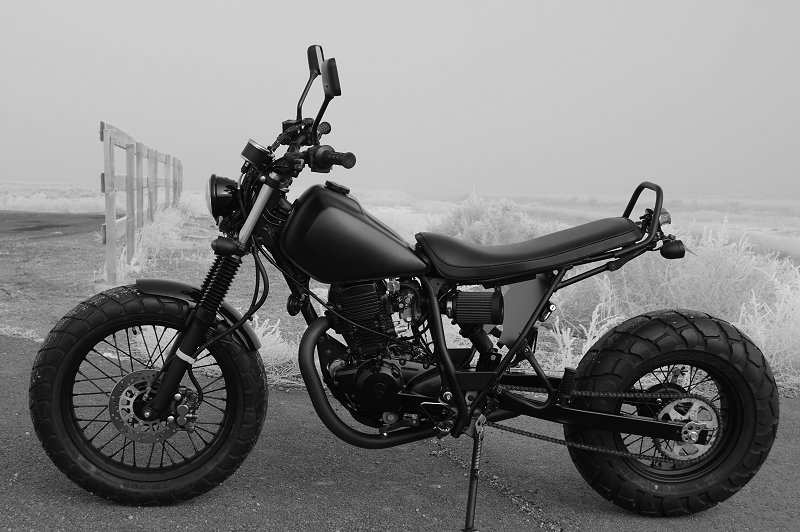
\includegraphics[width=\textwidth]{motor_original.png} \caption{Original image} %\label{fig:LPF} 
\end{subfigure}
\begin{subfigure}[b]{0.4\textwidth} 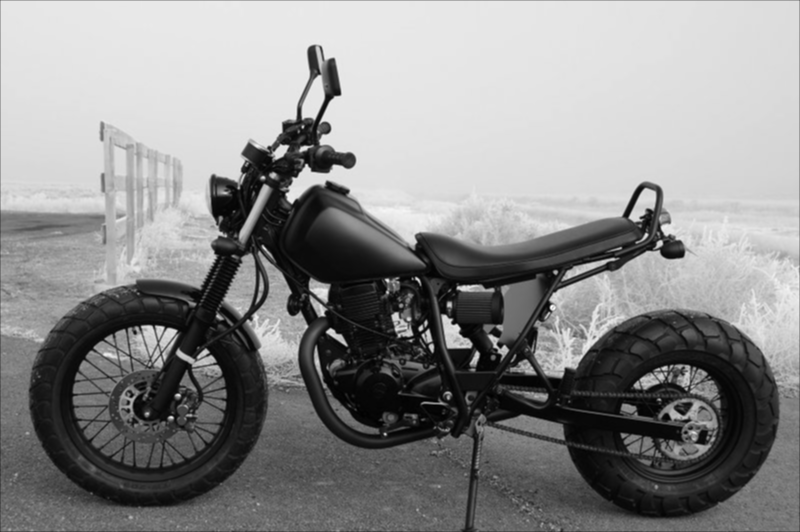
\includegraphics[width=\textwidth]{motor_direct.png} \caption{Low pass, direct}\end{subfigure}

\begin{subfigure}[b]{0.4\textwidth} 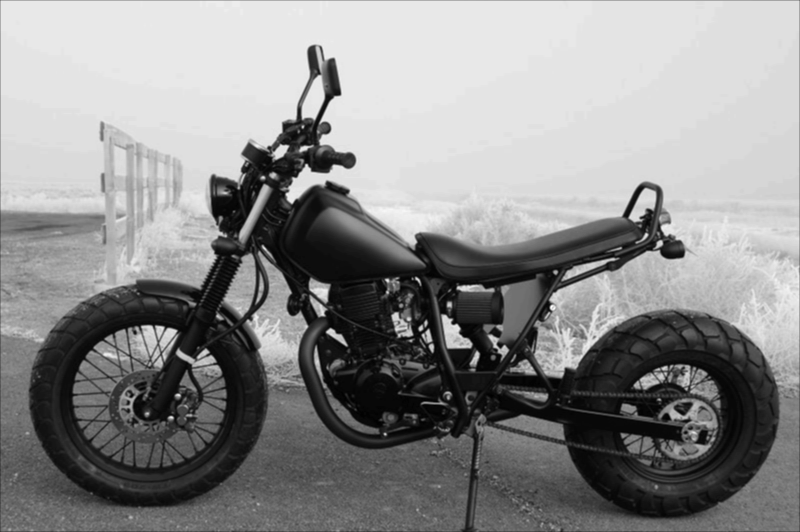
\includegraphics[width=\textwidth]{motor_lut_121.png} \caption{Low pass, LUT with $T_1$} %\label{fig:LPF} 
\end{subfigure}
\begin{subfigure}[b]{0.4\textwidth} 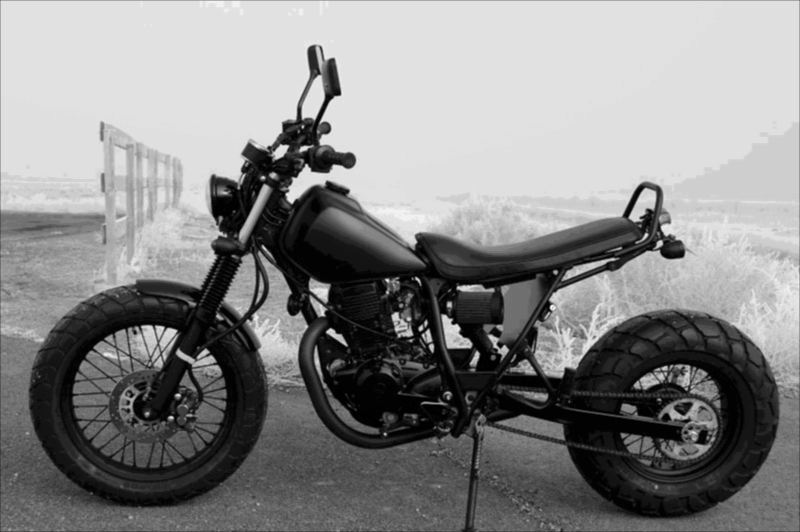
\includegraphics[width=\textwidth]{motor_lut_242.png} \caption{Low pass, LUT with $T_2$} \end{subfigure}
\caption{Comparison of filtered images}
%\label{fig:comp} 
\end{figure}
\end{frame}

\begin{frame}
\frametitle{An Approximate Decomposition}
\begin{beamerboxesrounded}[lower=eeks2,upper=eecks,
shadow=true]{IDEA}
%Idea: 
The more zeros in our filter the smaller the LUT. Can we decompose the (3$\times$ 3) filter $K$ in a better way? Consider:
$$
K=A*B
$$
where
$$A=
\begin{bmatrix}
a & b & 0\\
c & d & 0\\
e & f & 0
\end{bmatrix}
,
B=
\begin{bmatrix}
g & h & i\\
j & k & l\\
0 & 0 & 0
\end{bmatrix}
$$
\end{beamerboxesrounded}

\begin{itemize}
\item
Size of the LUT reduces from $2^{72}$ bytes to $2^{49}$ bytes before any truncation.
\item
We can solve the minimization problem
$$
\min (\|K-A*B\|_F + Total Edge Sum)
$$
\end{itemize}
\end{frame}

\begin{frame}
\frametitle{Approximate Decomposition Example}
\begin{figure}[htb]
  \begin{center}
  \mbox{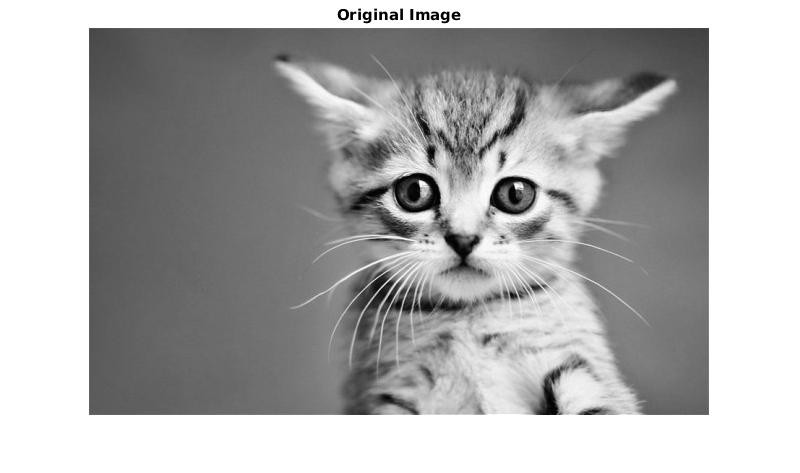
\includegraphics[height=1.3in]{kitten.png}}
   \mbox{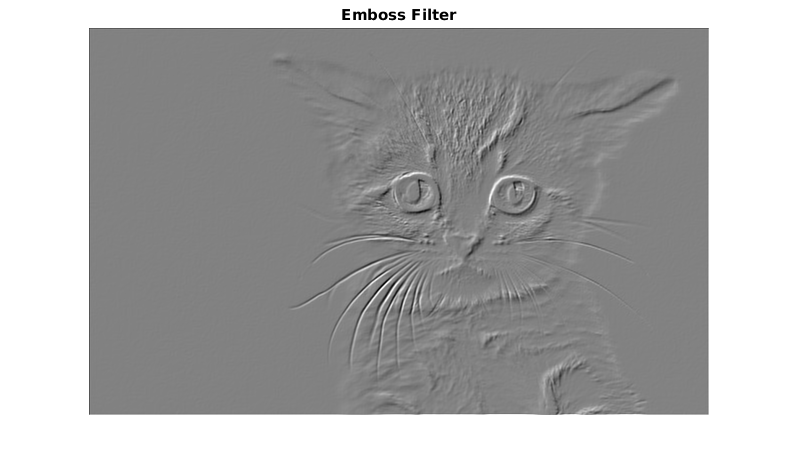
\includegraphics[height=1.3in]{kitten_Emboss.png}}
   
\end{center}
\end{figure}

$$
\arraycolsep=1.5pt\def\arraystretch{1.2}
K=\begin{bmatrix}
    -1 &   -1   &  0 \\
    -1   &  0   &  1 \\
     0   &  1  &   1
\end{bmatrix},
\arraycolsep=1.0pt\def\arraystretch{1.2}
A=
\tiny
{\begin{bmatrix}
  -0.000  & -0.000   & 0.000 \\
   -0.000   & 1.702  &  0 \\ 
    0.000    &     0   &      0
\end{bmatrix}}
,
B=
\tiny{\begin{bmatrix}

   -0.587 &  -0.587   &      0\\
   -0.587  &       0  &  0.587\\
         0   & 0.587 &   0.587
\end{bmatrix}}
$$
\begin{itemize}
\item
$\|K-A_T*B_T\|_F < 3.04*10^{-5}$
\end{itemize}

\end{frame}

\begin{frame}

\begin{table}[ht]
\begin{center}
\begin{tabular}{c|c|c|c|}\cline{2-4}
& Emboss & Low-Pass & Averaging \\\hline \multicolumn{1}{ |c| }{PSNR}
& 42.0500  & 71.0895 &  \\\hline
\multicolumn{1}{ |c| }{$l_{2}$ - error}  & 0.0079 & 2.7895e-04 &  \\\hline \multicolumn{1}{ |c| }{$max$ - error} & 0.0144  & 6.1630e-04 & \\
\hline
\end{tabular}
\caption{Comparison of errors}
\label{table:comparison_of_errors}
\end{center}
\end{table}
The errors are measured as such
\begin{itemize}
\item []
PSNR(A,B)$=20 \cdot \textrm{log}_{10} ( \frac{\textrm{MAX}_B}{\sqrt{\textrm{MSE}}} )$
\item[]
$l_2$-error(A,B)$=\sqrt{ \frac{ \sum_{i,j} \left( a_{ij} - b_{ij} \right)^2} {h \times w}}$
\item[]
$l_{\infty}$-error(A,B)$=\textrm{max}_{i,j} | a_{ij} - b_{ij}|$
\end{itemize}
\end{frame}




\begin{frame}\frametitle{Decomposing a Kernel Matrix by Rows}
\begin{itemize}
\item A kernel matrix $K_{n\times n}$ of \emph{any} rank can always be decomposed as
$$K = \left[\begin{matrix}1\\0\\\vdots\\0\end{matrix}\right]*[r_1] + \left[\begin{matrix}0\\1\\\vdots\\0\end{matrix}\right]*[r_2] + \cdots + \left[\begin{matrix}0\\0\\\vdots\\1\end{matrix}\right]*[r_n],$$
where $r_i$ is the $i$th row of $K$.
%\pause\item Also, convolving with one of the standard basis vectors of $\R^n$ is a vertical shift of pixels in the image, and does not require its own LUT.
\pause\item Essentially, this decomposition allows us to convolve our image by one row of $K$ at a time, and simply add the results at the end.
\pause\item If using LUTs, computation is reduced to $n$ look-ups and $n-1$ additions per pixel, with each LUT having $2^{8n}$ entries.
\pause\item Compare this to a single LUT, which requires only one look-up operation, but the table contains $2^{8n^2}$ entries!
\pause\item Even when $n=3$, this is the difference between one 4-zebibyte table ($\approx$1\% of one mole of bytes) and three 16MB tables!
\end{itemize}
\end{frame}

\begin{frame}\frametitle{Decomposing a Kernel Matrix by Rows}
\only<1>{\begin{figure}[h] 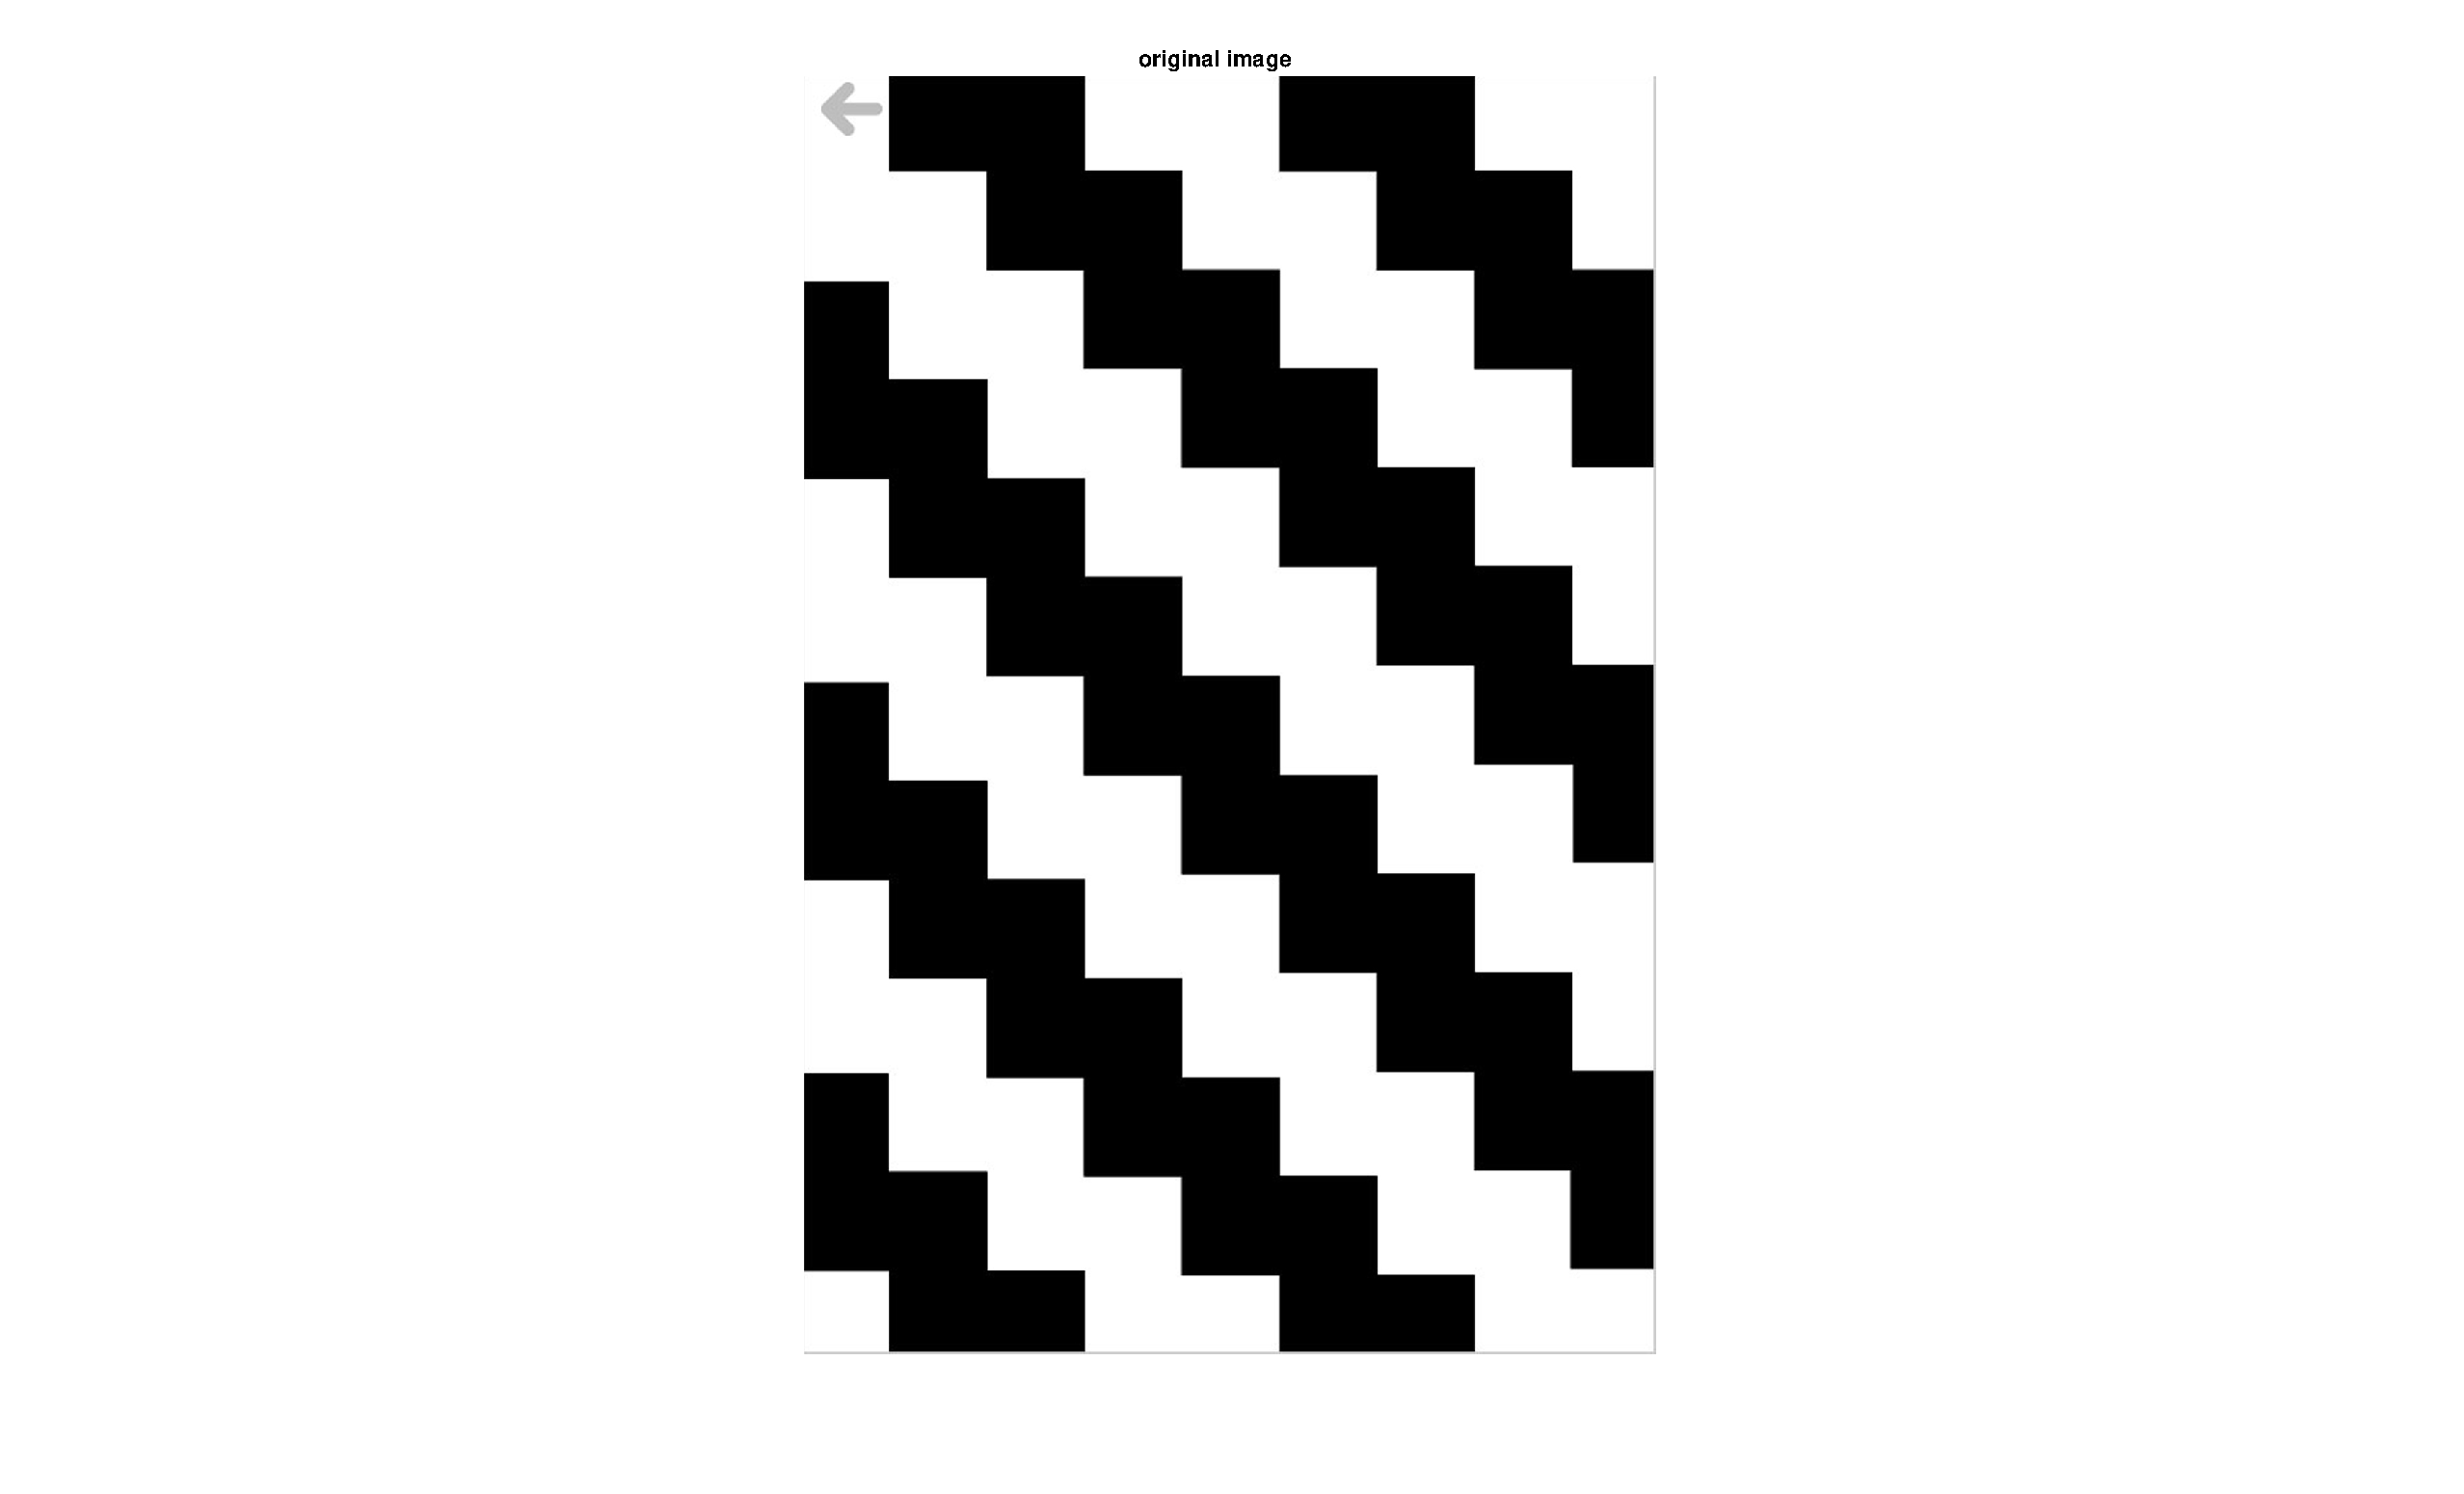
\includegraphics[width=280pt]{zigzag.eps} \caption{Original Image} \label{blah} \end{figure}}
\only<2>{\begin{figure}[h] 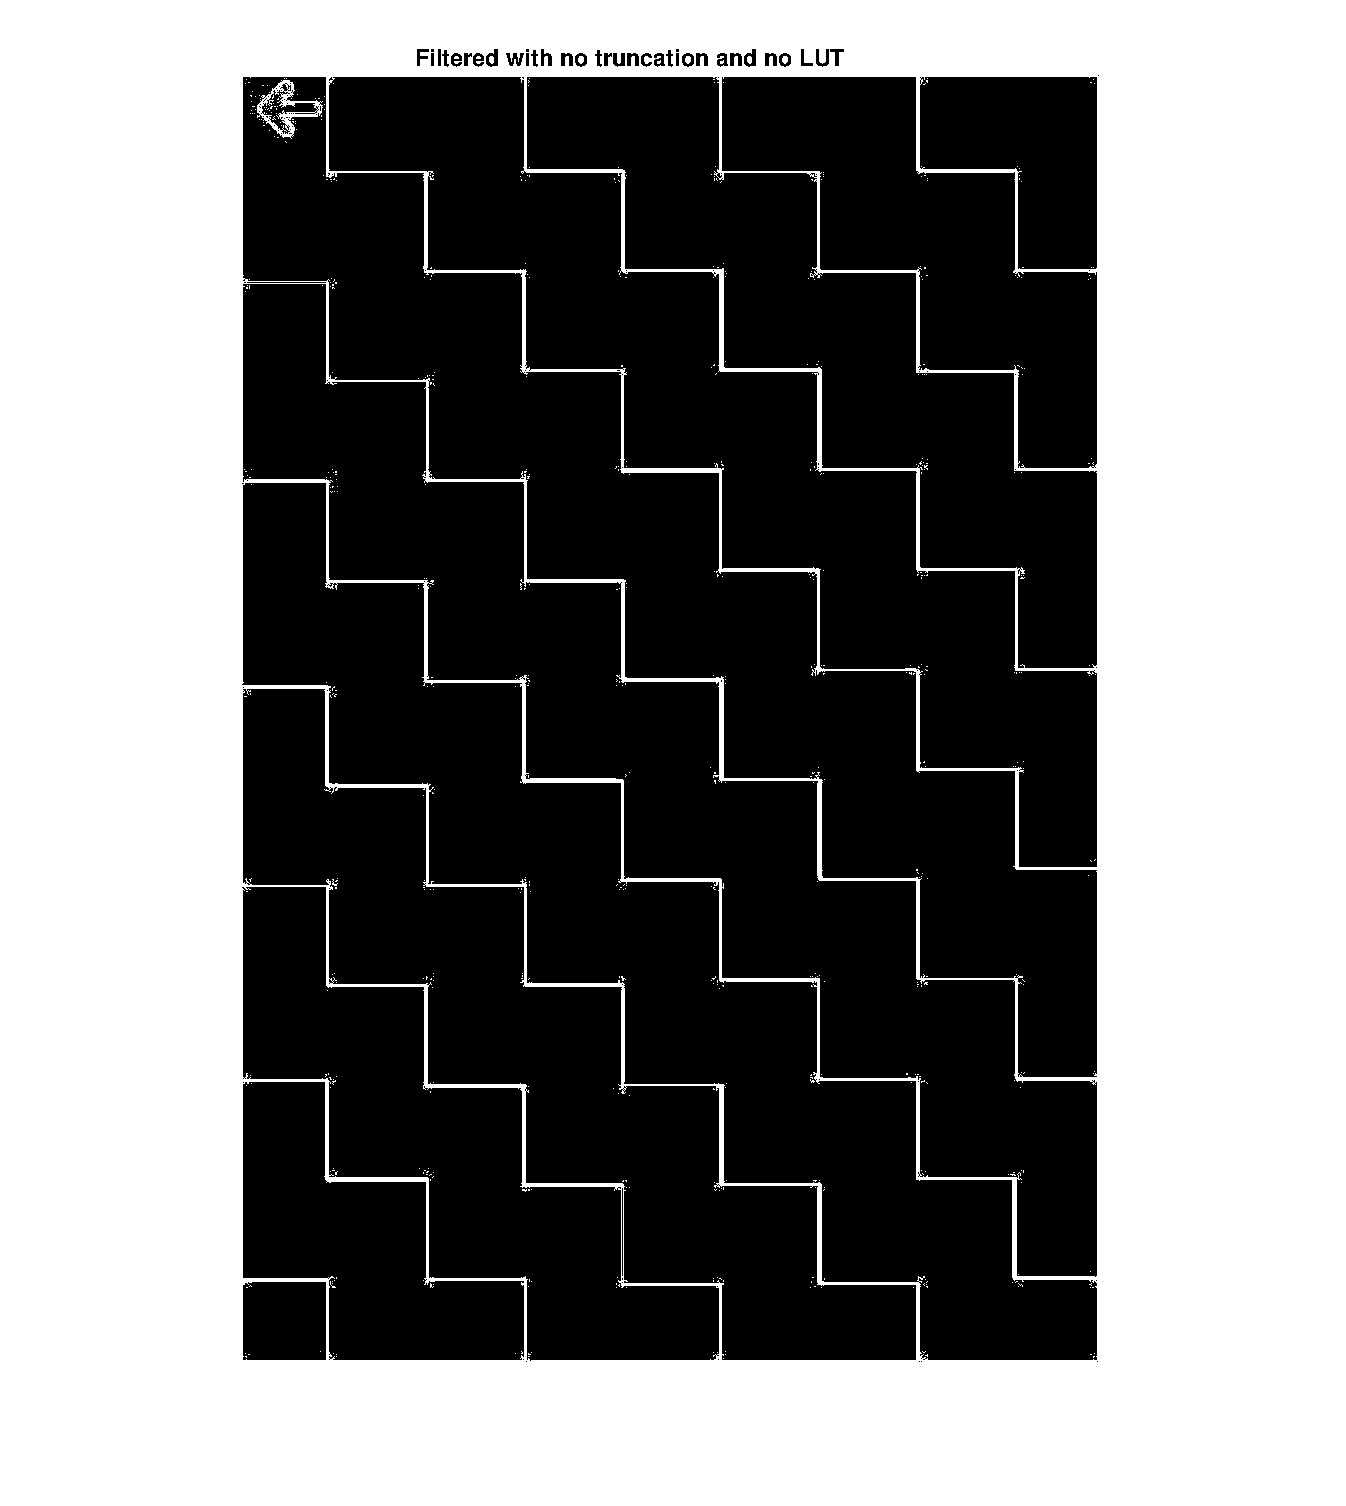
\includegraphics[width=140pt]{zigzag_HP.eps} \caption{Image after HP filter} \label{blahblah} \end{figure}}
\only<3>{\begin{figure}[h] 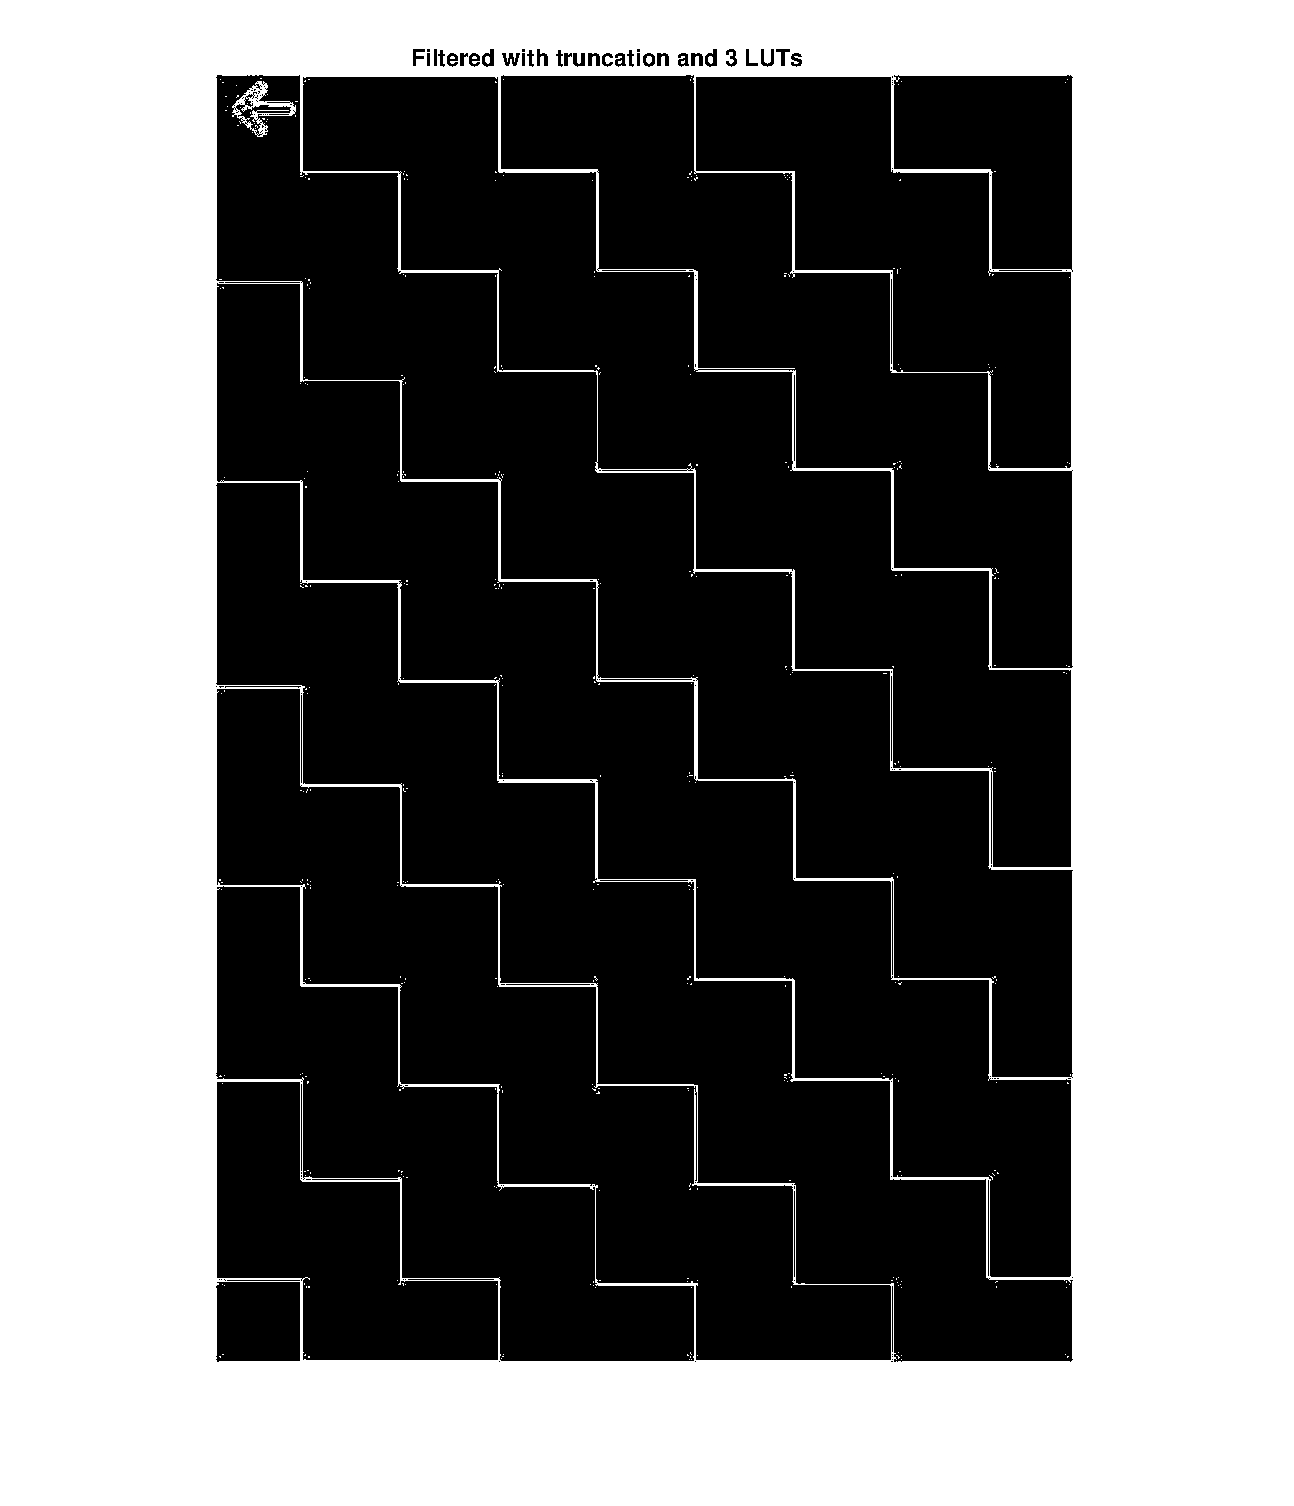
\includegraphics[width=140pt]{zigzag_HP_LUT_T.eps} \caption{Image after HP filter with 3 LUT's\\containing 16, 4096, and 16 entries} \label{blahblahblah} \end{figure}}
\end{frame}

\begin{frame}
\frametitle{Truncation and Blurring Filter (using Edge-detection filter)}
Observation
\begin{enumerate}
\item The truncation method can be used to reduce running time.
\item Truncation makes some errors such as staircase effects for blurring, but is decent for edge-detecting.
\end{enumerate}
\bigskip
\pause
\begin{center}
$\Downarrow$
\end{center}

\pause
\begin{beamerboxesrounded}[lower=eeks2,upper=eecks,
shadow=true]{Goal}
Take advantage of the truncation method avoiding staircase effects!
\end{beamerboxesrounded}
\end{frame}

\begin{frame}
\frametitle{Truncation and Blurring Filter (using Edge-detection filter)}

\begin{beamerboxesrounded}[lower=eeks2,upper=eecks,
shadow=true]{IDEA}
$I-L$ can be regarded as an edge-detection filter even though it is not a high-pass filter in general.
\end{beamerboxesrounded}

\begin{wrapfigure}{l}{0.3\textwidth}
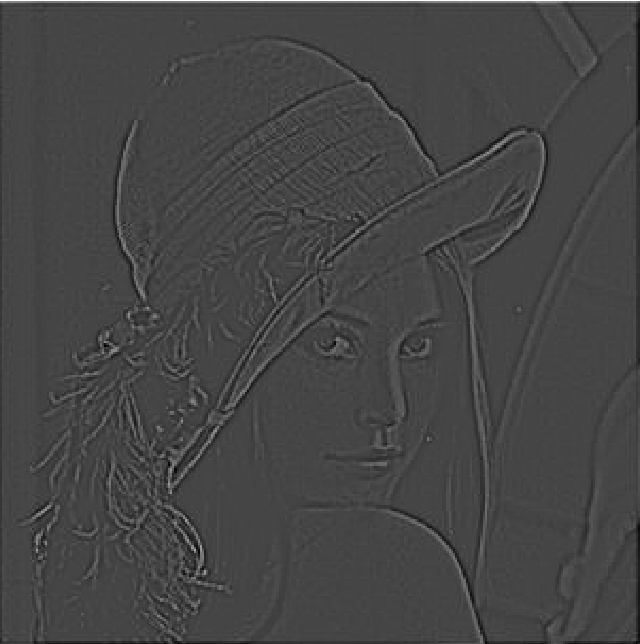
\includegraphics[width=0.9\linewidth]{I-LPF.png} 
\caption*{Example of $I-L$.}
\end{wrapfigure}

\bigskip

\pause

Strategy

\begin{itemize}
\item[1.] Let $L$ be given low-pass filter.
\item[2.] Set $H:=I-L$. 
\item[3.] Find $I-H(T)$ for a certain truncation $T$.
\end{itemize}
\pause
\begin{center}
$\Downarrow$
\end{center}

\pause
$$L\approx I-H(T)$$
\end{frame}

\begin{frame}
\frametitle{Truncation and Blurring Filter (using Edge-detection filter)}
Let $$L=
\frac{1}{8}
\begin{bmatrix}
0 & 1 & 0\\
1 & 4 & 1\\
0 & 1 & 0
\end{bmatrix} \mbox{ and } T=\left[
\begin{array}{ccc}
8 & 6 & 8 \\
6 & 4 & 6 \\
8 & 6 & 8
\end{array}
\right].$$

\begin{figure}[h] \centering 
\begin{subfigure}[b]{0.3\textwidth} 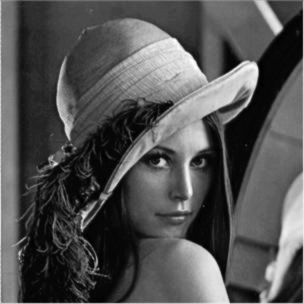
\includegraphics[width=\textwidth]{LPF.png} \caption{Low-pass filter, $L$} \end{subfigure}
\begin{subfigure}[b]{0.3\textwidth} 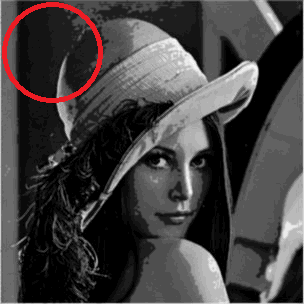
\includegraphics[width=\textwidth]{truncation.png} \caption{Truncation, $L(T)$} \end{subfigure}
\begin{subfigure}[b]{0.3\textwidth} 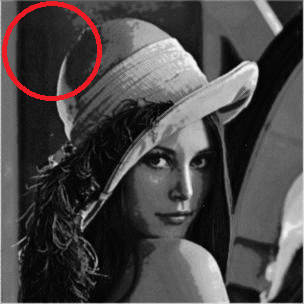
\includegraphics[width=\textwidth]{new.png} \caption{New Idea, $I-H(T)$} \end{subfigure}
\caption{Comparison of filtered images}%\label{fig:comp} 
\end{figure}

\end{frame}

\begin{frame}
 The table shows us how $L(T_i)$ and $I-H(T_i)$ are different from the low-pass filter $L=I-H$ for each $i$. $L(T_i)$ is Old and $I-H(T_i)$ is New in the table.

\begin{table}[ht]
\begin{center}
\begin{tabular}{c|c|c|c|c|c|c|}
\cline{2-7}  & \multicolumn{2}{|c|}{$T_{1}$} &
\multicolumn{2}{c|}{$T_{2}$} & \multicolumn{2}{c|}{$T_{3}$}
\\\cline{2-7} & Old & New & Old & New & Old & New \\\hline \multicolumn{1}{ |c| }{PSNR} &
38.12 & 39.58 & 30.80 & 32.84 & 22.59 & 25.59 \\\hline
\multicolumn{1}{ |c| }{$l_{2}$ - error} & 3.06 &  2.80 &  7.40 & 5.87 &
18.87 & 13.52 \\\hline \multicolumn{1}{ |c| }{$l_{\infty
}$ -
error} & 8.42 & 7.40 & 19.64 & 15.81 & 43.35 & 35.70 \\
\hline
\end{tabular}
\bigskip

\caption{Comparison of errors}
\end{center}
\end{table}
\end{frame}
\section{Further Directions}

\begin{frame}
\frametitle{Further Directions}
\begin{enumerate}
\item Refine convolution decomposition
%\item Compute trade-off between errors (due to truncation) and speed
\item SVD (singular value decomposition)
%\item Run further tests
%\item $5\times 5$ filter matrix
\end{enumerate}
\end{frame}

\begin{frame}
\frametitle{ }
\begin{center}
{\huge Thank you!}
\end{center}
% Thank the IMA and our mentor Dr. Wu
\end{frame}

\end{document}